\section{Why fitting a short running sum can fail on the next step}\label{sec:front}
A recurrent neural network (RNN) carries a state vector from one input to the next. Let $d\ge1$ be the number of state coordinates. At step $t\ge1$ let $x_t$ be the scalar input, $h_t$ the column of $d$ real state values, and $y_t$ the scalar output. Choose a coordinate $j$ from $1$ to $d$, let $e_j$ be the column with a one at $j$ and zeros elsewhere, and write $c=e_j^\top$ for its transpose. Multiplication by the fixed row $c$ reads coordinate $j$. With a $d$-by-$d$ transition matrix $A$ and an input-weight column $b$, the network is
\[
             h_0=0,\qquad h_t=Ah_{t-1}+b x_t,\qquad y_t=c h_t .
\]
There is no additive offset. Holding $A,b$ fixed over time gives the same update rule at every step.

Specify the target by a nonzero sequence of real coefficients $g=(g_0,g_1,\ldots)$. Its response at step $t$ is the convolution $\sum_{k=0}^{t-1}g_k x_{t-k}$, a weighted sum of the current and past inputs. The \emph{unit impulse} is the stream beginning with $1$ followed by zeros. The network's successive outputs on it are $cA^kb$ for integers $k\ge0$, with $A^0$ the identity matrix. By linearity, matching all streams for the first $H$ steps is equivalent to the $H$ identities $cA^kb=g_k$ for $0\le k<H$. We call $H$ the horizon and the first $H$ coefficients the prefix.

Let $S$ be the shift on sequences, defined by $(Sg)_k=g_{k+1}$. For a polynomial $p(z)=\sum_{i=0}^m p_i z^i$ of degree $m$ in a variable $z$, write $(p(S)g)_k=\sum_{i=0}^m p_i g_{k+i}$. The \emph{recurrence order} $r$ is the smallest degree of such a polynomial with leading coefficient one for which $p(S)g$ vanishes at every index. Thus $r$ terms determine the next by a fixed linear rule. For fixed $g$ and $j$, let $E(d,r,H)$ be the fewest entries of the initialized pair $(A,b)$ that must change to match the prefix. There are $D=d^2+d$ editable entries, each costing one edit if changed.

\begin{theorem}[Minimum edit count]\label{th:edit}
Fix the target independently of the initialization. Assume $d\ge r$, and draw $(A,b)$ from a joint distribution with a density on the real parameter space. With probability one, for every integer $H\ge1$,
\[
                         E(d,r,H)=\min\{H,d+r\}.
\]
Matching every horizon costs $d+r$ edits. For $d<r$, no such network matches every horizon.
\end{theorem}
Here \emph{with probability one} excludes a set of initial weights of volume zero. Continuous Xavier draws satisfy this assumption. The theorem provides a benchmark for finite binary64 draws, which have a discrete distribution. At $H<d+r$ a minimum-edit exact fit must fail on the next coefficient, since that coefficient requires one more edit. Conversely, let $\chi_A(z)=\det(zI-A)$ be the characteristic polynomial of $A$, where $I$ is the identity matrix and $\det$ the determinant. The Cayley--Hamilton identity $\chi_A(A)=0$ makes the network coefficients obey a recurrence of degree at most $d$. Their difference from the target obeys the recurrence given by $\chi_A(S)p(S)$ of degree $d+r$. Its first $d+r$ zeros force all subsequent terms to vanish.

For a running sum $g_k=1$ and $r=1$. One construction sets $cA=c$ and $cb=1$ by writing the observed row and one input weight. A second sets $b_j=1$ and changes column $j$ until $Ab=b$, so all input contributions lie on the line spanned by $b$. Both use $d+1$ edits at almost every starting point, or 33 of 1,056 entries at $d=32$. In the general construction, changing entries of $b$ matches a short prefix. Beyond $d$ coefficients, selected entries in one column of $A$ can also change its characteristic polynomial. Appendix~\ref{app:proof} gives the construction and lower bound, including networks whose output cannot observe every state direction.

\begin{figure}[htbp]
\centering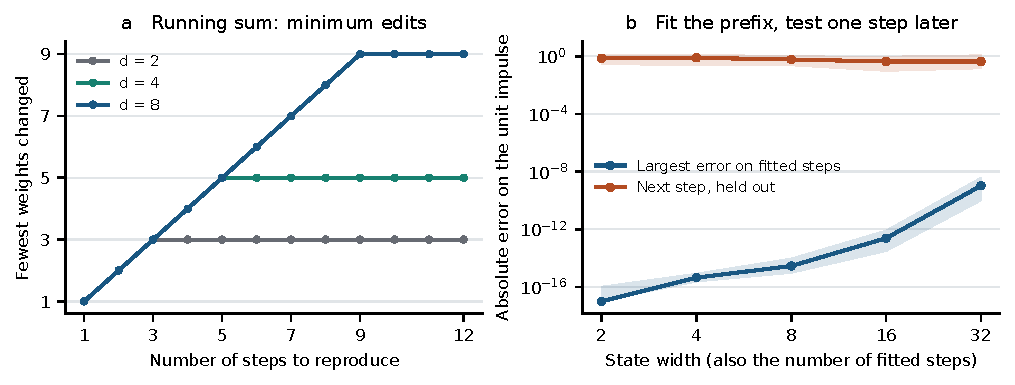
\includegraphics[width=\linewidth]{frontier.pdf}
\caption{A linear recurrent network stores $d$ numbers and returns one fixed state coordinate. At left, choose a number of steps on the horizontal axis. A point gives the fewest individual weights that must change to reproduce all those running sums, for the indicated state width. For example, at width four the cost stops at five edits. These points are exact theoretical values. At right, the horizontal axis is the number of state coordinates. We give each network an input of one followed by zeros and fit its input weights to the first $d$ outputs, all equal to one. The vertical axis gives absolute error on this sequence. Only the right panel aggregates trials: each point is a median across 64 random starts. The bands show the middle 50\% of these runs. The fitted error is the largest absolute error on the prefix. The unseen error is the absolute error on its next coefficient. Values below $10^{-17}$ appear at $10^{-17}$ on the logarithmic axis.}\label{fig:front}
\end{figure}

\section{Can a language model find the predicted edits?}\label{sec:writer}
For a target state $s_t$ at step $t$, choose a multiplier $\lambda$ on its previous value and an input gain $\gamma$. Starting at $s_0=0$, the target rule is $s_t=\lambda s_{t-1}+\gamma x_t$. A running sum has $\lambda=\gamma=1$. In each of six pairs we sent Astra the same initialized network, rule, fixed output coordinate and ordering of entries in the array. One request specified just a prefix and allowed scratch arithmetic. The other specified all horizons and prohibited tools. Each edit was an index and a replacement value. Neither request received test feedback. Table~\ref{tab:astra} reports all six pairs.

\begin{table}[htbp]\centering\small\setlength{\tabcolsep}{3.4pt}
\caption{Paired WSP requests for $s_t=\lambda s_{t-1}+\gamma x_t$, and a BP control given the same editable entries. Here $d$ is state width and $H$ is the short horizon and short edit count. Fit exact counts matching impulse coefficients out of $H$. Next gives the absolute error on coefficient $g_H$, also its single-output RMSE. WSP and BP agree to the three decimal places shown for Next. The last column counts all-horizon WSP edits.}\label{tab:astra}
\begin{tabular}{@{}lrr rr rr rr@{}}\toprule
&&&\multicolumn{2}{c}{Short WSP}&\multicolumn{2}{c}{Short BP}&&All-horizon\\
$(\lambda,\gamma)$&$d$&$H$&Fit exact&Fit RMSE&Fit exact&Fit RMSE&Next&WSP edits\\\midrule
$(1,1)$ & 4 & 2 & 1/2 & $7.85\times10^{-17}$ & 1/2 & $1.57\times10^{-16}$ & 0.156 & 5\\
$(1,1)$ & 5 & 3 & 2/3 & $1.28\times10^{-16}$ & 0/3 & $1.24\times10^{-15}$ & 1.528 & 6\\
$(1,1)$ & 6 & 4 & 2/4 & $3.14\times10^{-16}$ & 0/4 & $2.10\times10^{-14}$ & 0.938 & 7\\
$(-1/2,2)$ & 4 & 2 & 1/2 & $2.21\times10^{-14}$ & 1/2 & $2.20\times10^{-15}$ & 0.630 & 5\\
$(1/2,-1)$ & 5 & 3 & 2/3 & $3.20\times10^{-17}$ & 0/3 & $1.57\times10^{-16}$ & 1.514 & 6\\
$(-1,1/2)$ & 6 & 4 & 2/4 & $6.21\times10^{-17}$ & 0/4 & $9.36\times10^{-15}$ & 0.018 & 7\\
\bottomrule
\end{tabular}\end{table}

All six all-horizon replies set $cA=\lambda c$ and $cb=\gamma$. Substitution into the update proves the target recurrence for every real stream. Each also reproduced all 512 central streams of length eight and all 512 outer streams of length 64 with zero RMSE. The short replies used $H$ edits. Their decimal values met the requested absolute tolerance of $10^{-9}$ on every fitted impulse coefficient, and each missed the next coefficient. The theorem predicts their edit \emph{count} for a real exact fit. The numerical replay measures agreement after rounding.

Two checks separate this result from the behavior of one solver. At width eight, a numerical solve for the input weights on eight impulse coefficients gave a median maximum prefix error of $2.8\times10^{-15}$ and a median next error of $0.588$ over 64 starts (Figure~\ref{fig:front}b). An adaptive gradient method also learned an exact running sum. In a scalar cell with transition weight $a$, input weight $b$ and output equal to its state, a unit gradient step on half the squared final error for the labeled stream $(1)$ sets $b=1$ in real arithmetic. Next choose the input stream $(1,-a)$ and hold its values fixed while differentiating. The output has derivatives $(1,0)$ with respect to $(a,b)$ and its target is $1-a$. A second unit step sets $a=1$. Repeating each update once to accommodate rounding gave exactly $(a,b)=(1,1)$ in 256 of 256 binary64 Xavier draws, with zero RMSE on 512 outer streams per draw.

For a matched numerical control, we disclosed the locations of the WSP edits to BP, froze all other entries and used 800 Adam steps followed by up to 1,000 BFGS iterations. The short control received the same $H$ impulse labels. For the all-horizon control we supplied the first $d+1$ impulse labels, enough to certify an \emph{exact} fit for an order-one target at width $d$. On each of the six outer tests WSP attained 512/512 complete streams with zero RMSE. BP attained 0/512 in each case, with shell RMSE between $1.02\times10^{-13}$ and $1.44\times10^{-11}$. The archive includes all six pairs at full precision.
